\chapter{General discussion}
\label{chap:general-discussion}

The aim of this chapter is to bring together the different aspects of the research carried out (Chapters \ref{chap:eodal}-\ref{chap:drc}) within the framework of a landscape-scale prototype and to discuss its applications, limitations and possible further research questions. However, the scientific discussion of the individual research chapters is not repeated here. Please refer to the relevant discussion subsections in the previous chapters.

\section{A prototype for landscape-scale phenotyping}
Figure \ref{fig:oa-disc-prototype} shows a sketch of how the individual research components can be transferred to a landscape level prototype to quantify winter wheat growth and development.

The main data sources for the prototype are environmental covariates, mainly air temperature, and high resolution optical satellite imagery from the \gls{S2} mission. The necessary calibration of the prototype is mainly based on field phenotyping data, which encode the relationships between development and growth (see Chapter \ref{chap:insights}) and between plant growth and environmental conditions (Chapter \ref{chap:drc}). These calibration data thus represent the physiological and phenological knowledge of G $\times$ E interactions in crops in general and wheat in particular.

\subsection{Components}
Using the calibration and the two data sources, the functionality of the prototype can now be demonstrated in three components.

\paragraph{Components1 -- Timing and duration of key phenological stages}
The first step is to determine the timing of key phenological development stages as described in Chapters \ref{chap:phemology} and \ref{chap:insights}. This is important to determine the onset and duration of the \gls{SE} period, which was the main focus of this thesis due to its importance in grain yield formation, as explained in Chapter \ref{chap:introduction}. The phenology model uses day length and weather data and has a coarse spatial resolution (km scale) due to the relatively coarse resolution of most meteorological data products at the landscape scale. The timing extracted from the phenology model will therefore limit the period over which satellite data should be considered.

\paragraph{Component 2 -- Trait retrieval from satellite imagery}
Once the relevant time period has been extracted from the phenology model, satellite data are searched and converted to \gls{GLAI} using physiological and phenological priors from field phenotyping as described in Chapter \ref{chap:insights} using RTM inversion and the software \gls{EOdal} (Chapter \ref{chap:eodal}). Thus, at $n$ times, where $n$ is the number of cloud-free \gls{S2} scenes, \gls{GLAI} estimates are available at 10 $\times$ 10 m spatial resolution. This allows spatial detail to be resolved, e.g. on within-field heterogeneity, which, as noted above, is not available from the temperature data. The \gls{GLAI} estimates based on the \gls{S2} data are thus snapshots of the apparent growth conditions.

\paragraph{Component 3 -- Reconstruction of growth}
Using the \gls{S2} \gls{GLAI} observations and air temperature data for a second time, the growth dynamics in the \gls{SE} period can be modelled in hourly or daily resolution in a final step, as described in Chapter \ref{chap:drc} using \gls{DRC}s. This combines the high temporal resolution of the temperature data is combined with the spatial detail of the \gls{S2} \gls{GLAI} observations. Not only is the physiological knowledge from the field phenotyping encoded here, but the uncertainty propagation performed in Chapter \ref{chap:uncertainty} is also used to model growth and development during the \gls{SE} period.

\begin{figure}[H]
    \centering
    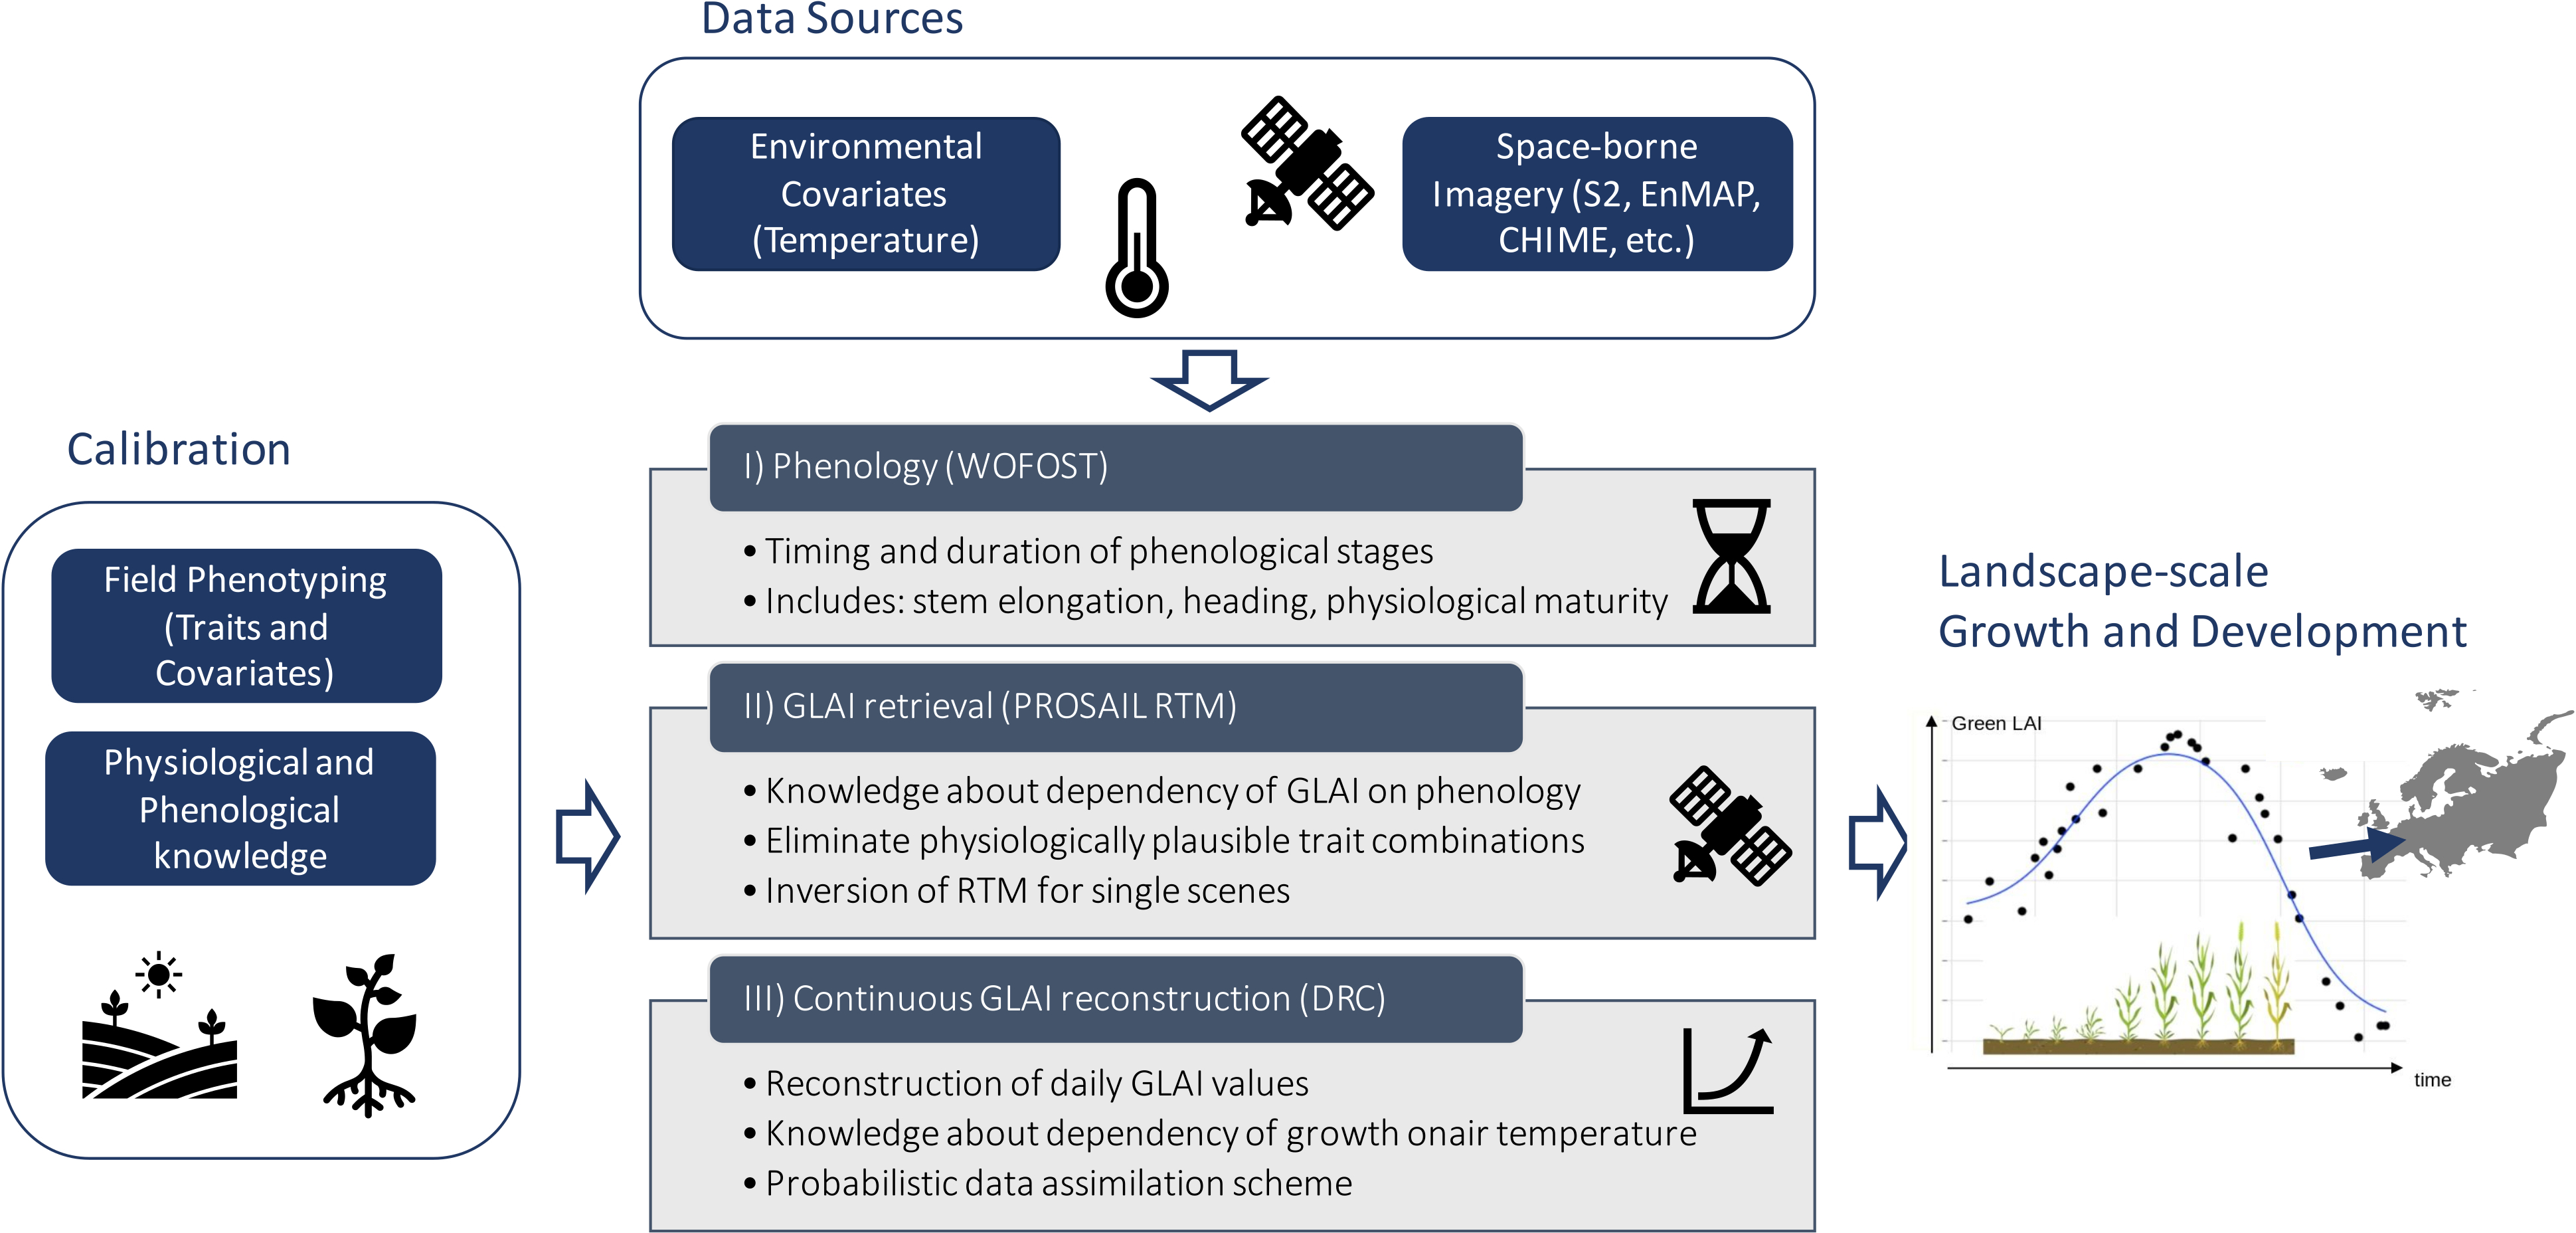
\includegraphics[width=\textwidth]{07-Discussion/img/prototype.jpg}
    \caption{The proposed prototype for landscape scale phenotyping of winter wheat growth and development as a key outcome of this thesis.}
    \label{fig:oa-disc-prototype}
\end{figure}

The prototype composed of these three components thus allows the quantification of winter wheat growth and development at the landscape scale, for example in the Swiss Plateau, with a spatial resolution of up to 10 m and a temporal resolution of up to one hour. Furthermore, by combining satellite, meteorological and in-situ data, the prototype can be considered as a true \gls{EO} system. At the same time, the quantification of growth through \gls{GLAI} values and development through phenological stages means that the prototype fulfils the definition of a phenotyping system.

The strength of the system presented here clearly lies in the linking of two disciplines, but also in the seamless integration of different components. Together they provide an integrated, holistic view of plant growth and development. This enables specific applications which are outlined in the following sections.

\subsection{Applications}
The prototype can effectively address the two pathways of agricultural transformation mentioned in Section \ref{sec:intro-motivation} to overcome the current challenges of negative environmental impacts of agricultural production, while helping to meet the increased demand for food and biomass.

\paragraph{Decision support and policy advice}
The phenotyping prototype presented is in line with multilateral initiatives such as \gls{GEOCLAM} or the European Union's Joint Research Centre MARS Bulletin with its European Crop Monitor \citep{van_der_velde_use_2019}, which aim to provide traceable, actionable insights to stakeholders in agriculture \citep{whitcraft_no_2019}. As the prototype is based on open satellite and, at least in most cases, readily available temperature data and rather simple but physiologically meaningful models, it appears well suited for further operationalisation and near real-time delivery of agronomically relevant information. Near-real-time information on the development and growth of stable crops such as wheat is arguably crucial for informed decision making, e.g. to reduce excessive fertiliser run-off \citep{argento_linking_2022} or for policy advice on potential crop failures and food shortages \citep{becker-reshef_strengthening_2020}. In this way, the scientific efforts of this thesis could contribute to increasing the resilience of the agricultural sector as a whole.

\paragraph{Research and breeding}
The phenotyping prototype also has potential applications in crop science, breeding and variety testing: in the future, in addition to small-scale field phenotyping trials, experiments could be conducted at the landscape scale on ``real'' farms to better investigate effects such as soil, topography or microclimate. This is in line with the objectives of the European project EMPHASIS\footnote{\url{https://emphasis.plant-phenotyping.eu/}}, which aims to establish a pan-European, cross-scale phenotyping infrastructure for more sustainable and resilient food production \citep{pieruschka_plant_2019}. Landscape-scale phenotyping could not only deepen the scientific understanding of plant-environment interactions, but also contribute to accelerated variety testing and provide breeders with an additional tool for selecting and evaluating breeding lines.

\section{Answers to research questions}
With the prototype (Figure \ref{fig:oa-disc-prototype}) the three research questions outlined in section \ref{sec:intro-obj-rj} can be addressed.

\subsection{How can field phenotyping and spaceborne remote sensing data be combined to allow up-scaling of physiological knowledge from field phenotyping to the landscape-scale?}
This thesis has identified two ways of combining field phenotyping and spaceborne remote sensing data. The first way is to use field phenotyping data as prior knowledge to constrain \gls{RTM} simulations as shown in Chapter \ref{chap:insights}, and to fill temporal gaps and remove outliers using \gls{DRC}s to reconstruct hourly or daily \gls{GLAI} trajectories from single \gls{S2} observations (Chapter \ref{chap:drc}). This is a confirmation of the initial hypothesis stated in Chapter \ref{chap:introduction}. While the first way directly addresses the workflow of remote sensing retrieval and time series reconstruction, the second way is about using field phenotyping data to parameterise phenological models (Chapter \ref{chap:phemology}), which in turn are used to select relevant satellite imagery and quantify the timing of key developmental stages such as the end of heading. It is thus a more indirect way of incorporating field phenotyping data into an \gls{EO} approach that allows for quantification of development.

The physiological basis of the approach, together with the physically based \gls{RTM} and mechanistic phenological model used, allows us to confidently claim that the results of the phenotyping prototype are valid for the entire Swiss Plateau as a landscape unit. This is because the laws of biology and physics are universally applicable and the calibration datasets are assumed to be representative of the Swiss Plateau in terms of climate, day length and management. In other words, plants all over the world function according to the same biophysical and biochemical mechanisms and differ only in the range of values of the model parameters, i.e. those processes that we cannot, or cannot well, represent in the model using physical and biological formulae. The geographical applicability of model parameter sets is then only a question of the representativeness of the underlying calibration data and the consistency of management plans. Concepts such as the Global Agro-Environmental Stratification zones \citep{mucher_new_2016} can give some indication of how the presented prototype could be used at European level, for example.

As a result, both pathways identified above allow knowledge and concepts to be scaled up from field phenotyping to the landscape scale.

\subsection{Can a landscape-scale phenotyping approach provide accurate, physiologically based and traceable insights into winter wheat growth and development?}
The quantification of uncertainties (see Chapter \ref{chap:uncertainty}) fulfils the requirement for traceability (Section \ref{sec:intro-obj-rj}). The integration of prior knowledge from field phenotyping into the \gls{GLAI} retrieval process in step 2, as well as into the parameterisation of \gls{DRC}s in step 3, fulfils the requirement for physiological plausibility (see also the individual scientific discussions in Sections \ref{sec:insights_discussion} and \ref{sec:drc_discussion}). The accuracy of the methodology has been demonstrated using multi-year, independent in-situ data for phenological development (RMSE for heading date: 2 days, Chapter \ref{chap:phemology}) and GLAI (smallest relative error: 13\%, Chapter \ref{chap:drc}). The relative standard uncertainty in remotely sensed \gls{GLAI} values can take up to 5\% depending on the development stage of the crops (Chapter \ref{chap:uncertainty}), which translates into an uncertainty in the timing of \gls{LSP} events in the magnitude of a few days.

As the uncertainty budget is still incomplete, i.e. it is likely to be higher than the figures reported here (see the discussion in Section \ref{sec:unc_discussion}), and the uncertainty in field phenotyping data has not been addressed in this work, the research question can therefore be answered in the affirmative, with some reservations. Further quantification of the uncertainty is, however, clearly necessary, both in the satellite imagery and in the field phenotyping data. In addition, depending on the application, it should be clarified which uncertainty range is considered acceptable. For breeding experiments, this is probably much narrower than for large-scale biomass estimates.

\subsection{What are the potentials but also the limitations and challenges of such a landscape phenotyping approach?}

The prototype allows the study of G $\times$ E interactions that could not be fully addressed by small-scale field phenotyping experiments. These include effects of changes in soil properties or topography that are spatially continuous and affect plant growth and development through soil water availability, exposure to wind and sunlight, or nutrient availability. In addition, the \gls{GLAI} estimates can be converted to biomass \citep{aase_relationship_1978} and -- in perspective -- grain yield, which are arguably important agronomic traits for decision making and policy advice. Accurate modelling of these traits will therefore not only advance the science behind \gls{EO}-based applications for agriculture, but also help to meet the needs of a growing world population.

The main obstacle to this potential is the lack of in situ data: Management data, in particular the sowing date or the variety used, is essential agronomic information that is not yet available on a large scale. In many countries, including Switzerland, the management data that the state is obliged to collect and publish include the main crop, but no further management data. In addition, research data from field phenotyping and variety testing, which are key to calibrating models, are often not publicly available. When they are, the data are often not standardised and poorly documented, so it is not clear how the data were collected and what the uncertainties are.

From a modelling perspective, there is room for improvement in the representation of canopy structure and morphology, which would further increase physiological plausibility. This is related to the discussion on the representation of vertical gradients in leaf number and \gls{Cab} in Chapter \ref{chap:insights}. Canopy vertical gradients also address other research questions, such as differences in the interception of incoming solar radiation between sunlit and shaded leaves under direct and diffuse light conditions \citep{he_development_2013}. Approaches using multiple vertically stacked canopy layers would greatly facilitate the representation of gradients and could be a viable method for modelling, for example, the succession of senescence within a canopy.

Another limitation of the prototype is its spatial resolution of currently 10 m. This can cause spectral mixing problems close to field boundaries and make it difficult to resolve small-scale details such as flower strips, hedges or individual trees within a parcel. For small plots, it may not be possible to find a pure pixel, i.e. a pixel that is not affected by spectral mixing. \cite{meier_assessments_2020} found that, at a spatial resolution of 10 m, up to 6.4\% of all parcels (0.49\% of the total agricultural land area) were lost due to the lack of pure pixels, and for up to 50\% of the fields (10.53\% of the total agricultural land area) no site-specific agricultural applications were possible due to the small number of pure pixels ($\le$ 50 pixels). These figures were reported for Bavaria, which has a comparable average field size (1.6 ha) to Switzerland (1.4 ha) and a similar agricultural land use pattern. A solution to this problem could be the use of higher resolution data, such as from the Planet Labs$^{\circledR}$ constellation, with a pixel size of less than 5 m. In Samuel Wildhaber's master's thesis, it was shown that such high resolution data have potential for agricultural applications and could outperform \gls{S2} data when it comes to representing small-scale detail \citep{wildhaber_assessing_2023}. At the same time, unlike \gls{S2}, the data is proprietary and therefore more expensive to acquire. Deep learning based super-resolution may therefore be a more viable option to improve the spatial detail available from \gls{S2}, but research carried out by Julian Neff as part of his Master's thesis suggests that more effort may be required to achieve satisfactory results.

\section{Open questions}
\label{sec:disc-open-questions}
\subsection{Spatial or temporal detail?}
In Switzerland, the \gls{S2} constellation provides a temporal resolution of 3 to 5 days, depending on orbit coverage \citep{pazur_national_2022}. However, prolonged cloud cover can significantly reduce the number of images available, leaving critical developmental stages uncovered. In addition, undetected clouds and shadows add to the image noise, as the delineation of clouds and their shadows is highly uncertain due to spectral mixing effects, as discussed in Chapter \ref{chap:uncertainty}. The assimilation of \gls{DRC}-based hourly or daily growth rates and \gls{S2} observations has been proposed as a solution to this problem (Chapter \ref{chap:drc}). However, the cloudy spring of 2023 showed that even such sophisticated data assimilation schemes are limited by the number of satellite observations.

Data fusion approaches have therefore been proposed in the scientific literature. These include the fusion of different sensor types, such as different optical platforms or optical and \gls{SAR} data \citep[for example]{pipia_fusing_2019, lobert_mowing_2021}. Here, two strategies have been identified: The first is to increase the number of images by including coarse resolution observations from Landsat (30 m spatial resolution), \gls{MODIS} (250 m) or \gls{S3} (300 m) as suggested, for instance, by \cite{zhou_reconstruction_2020}. These data are also freely available, but lack significant spatial detail, as can be seen in Figure \ref{fig:discussion-l9-vs-s2}. Here, a Landsat-9 image at 30 m resolution is contrasted with an S2 image at 10 m resolution taken on the same day in June 2022 over Witzwil in western Switzerland, where the field size is almost 10 times larger than the Swiss average (13 ha, \cite{perich_pixel-based_2023}). In figure \ref{fig:discussion-l9-vs-s2}, it is clearly visible that the fields appear much more blurred at a resolution of 30 m. In addition, \cite{meier_assessments_2020} estimated that at 30 m, over 40\% of the fields no longer have a pure pixel. The second strategy is therefore to use higher resolution data than \gls{S2}, such as the Planet Labs$^{\circledR}$ data \citep[for example]{sadeh_fusion_2021}. However, this comes at the cost of increased financial burden and the need to use proprietary imagery. The fusion of \gls{SAR} data, which is attractive because of the cloud penetrating ability of the microwave radiation emitted, poses the challenge that the radiative properties in this spectral region differ significantly from optical data. Nevertheless, \cite{bai_could_2020} and \cite{villarroya-carpio_sentinel-1_2022} showed that \gls{SAR} coherence, i.e. the correlation coefficient of interferometric phase changes between single \gls{SAR} acquisitions, is correlated with \gls{NDVI} and is useful for agricultural applications.

It is clear that the use of Landsat or \gls{S3} data alone is not a realistic option for Switzerland, given the small size of the field plots. The open question, however, is what kind of data source should be used to fill the gaps. Is it really necessary to use expensive, proprietary data with high spatial and temporal resolution, which also increase storage requirements and computing time, or do coarse spatial resolution data such as \gls{S3} not nevertheless contain a certain amount of information about the crops that could be used for assimilation, for example? This ultimately comes down to the research question: What is more important -- spatial detail, temporal resolution, or both? A systematic comparison of the different platforms and sensors and their applicability for landscape phenotyping is certainly needed to provide answers.

\begin{figure}[H]
    \centering
    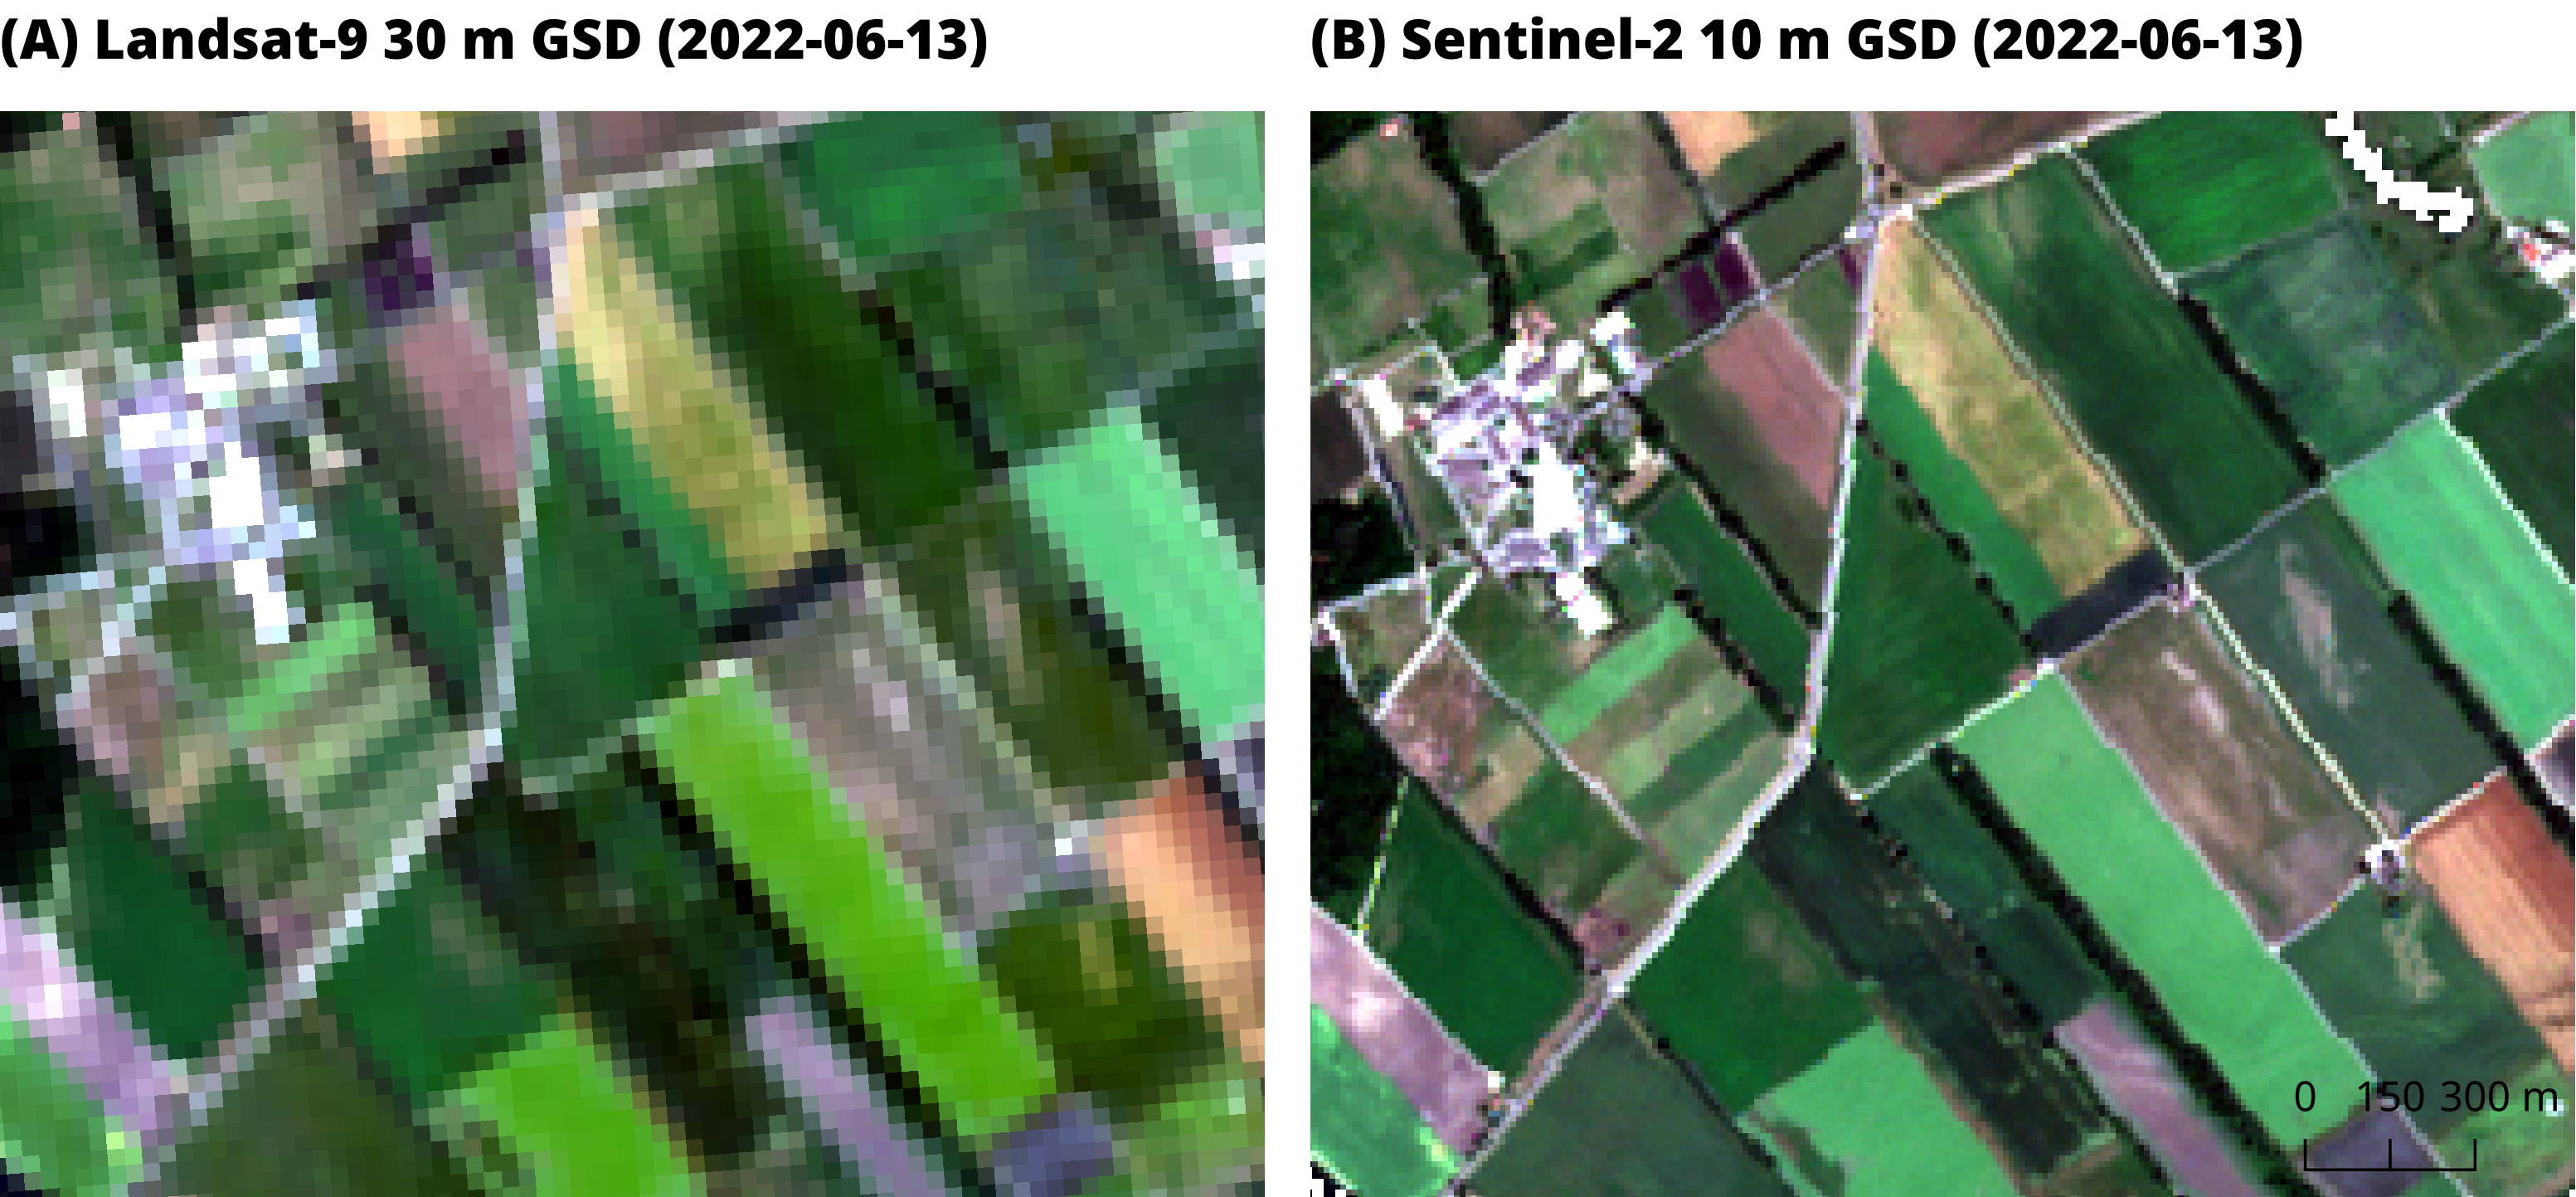
\includegraphics[width=\textwidth]{07-Discussion/img/comparison_l9-s2_witzwil22.png}
    \caption{Comparison of true-colour Landsat-9 30 m ground-sampling distance (GSD) and Sentinel-2 10 m GSD imagery acquired on 2022-06-13 of agricultural areas around Witzwil, Switzerland.}
    \label{fig:discussion-l9-vs-s2}
\end{figure}

\subsection{What are the limiting factors?}
In the Chapters \ref{chap:insights} and \ref{chap:drc} air temperature is considered as the main driver of plant growth \citep{porter_temperatures_1999}. By growth we mean the increase in \gls{GLAI} which -- during the \gls{SE} period -- correlates with the accumulation of dry matter, i.e. dry biomass (see Figure \ref{fig:ww-growth-development} and \cite{aase_relationship_1978}). \cite{monteith_climate_1977} points out that changes in leaf area are mainly controlled by temperature and soil water availability. Situations where wheat growth is water limited may become more relevant in the future due to climate change, even in Switzerland \citep{holzkamper_spatial_2015}. Currently, the prototype does not consider soil water availability, as this covariate is more difficult and costly to measure and is therefore often missing at larger spatial scales. Remotely sensed topsoil moisture \citep{lobell_moisture_2002, sadeghi_optical_2017} and hydrological modelling of surface water and energy balance \citep{penman_natural_1948, priestley_assessment_1972, shuttleworth_simplified_1978} could provide this information at larger spatial scales. However, the question remains whether leaf area dynamics are more controlled by temperature or water availability, as high temperatures tend to decrease soil moisture. This decrease is due to positive, non-linear feedback loops between air temperature, water vapour pressure deficit, evapotranspiration, soil moisture and temperature, and latent and sensible heat fluxes \citep{webber_diverging_2018, garcia-garcia_soil_2023}. Thus, further research on the ecophysiological processes governing the plant-soil-atmosphere continuum to identify the limiting factors for crop growth in terms of \gls{GLAI} dynamics at the landscape scale seems promising to uncover the underlying mechanisms. Another question that, to the best of our knowledge, remains largely unanswered is the effect of water availability on phenology.

An additional environmental covariate not considered in this thesis is global radiation, more specifically the fraction of absorbed \gls{PAR}, FAPAR. \cite{monteith_climate_1977} suggests modelling dry matter accumulation in terms of absorbed radiation and the efficiency with which the input solar radiation is converted into carbohydrates. The amount of radiation absorbed in turn depends on leaf area dynamics, the drivers of which have been outlined above. In an attempt to provide a unified formalism for describing crop growth in terms of leaf area \textsl{and} biomass throughout the crop development cycle, \cite{goudriaan_mathematical_1990} developed a prototype of what would become light use efficiency models \citep{gitelson_productivity_2015}. Apart from these considerations, too little radiation during meiosis, i.e. the production of gametes with the correct number of chromosomes, could lead to sterile flowers and thus reduce grain yield in winter wheat. Lack of radiation during meiosis, which occurs during booting, caused significant yield losses in France in 2016 \citep{le_gouis_how_2020}. This finding is in line with results from Spain and Mexico in spring durum \citep{villegas_daylength_2016}. To provide a more sophisticated perspective on leaf area and dry matter characteristics and ultimately grain yield, the use of light use efficiency models such as \gls{SAFYE} \citep{ma_wheat_2022} therefore seems promising as the next evolutionary step of the prototype.

Finally, the effects of management on plant growth and development, such as fertilisation, pesticides and growth regulators, should not be forgotten. This actually addressed the central question of whether M or E is more central at the landscape scale, i.e. whether plant growth and development is mainly driven by environmental covariates or farm management decisions.

\subsection{How to represent time?}

Time is an essential component in the description of dynamic processes such as growth and development. The choice of time axis is therefore critical, especially as there are different possibilities for plants. From an agronomic perspective, \gls{DAS}, \gls{GDD}s and \gls{BBCH} stages are commonly chosen time axes. However, from the remote sensing data, calendar dates are inevitably the first choice. As shown in Chapter \ref{chap:phemology}, \gls{DAS}, like calendar dates, are not very meaningful, as phenological development varies greatly from year to year and also shows great spatial variability within small spatial units. \gls{GDD}s take into account the temperature dependence of plant growth, as mentioned above, and can also be used to narrow down phenological macro-stages (see Chapter \ref{chap:insights}). However, the disadvantage of \gls{GDD}s is that they only work if the exact sowing date is known, which is often not the case. In addition, the link from \gls{GDD}s to phenological development is implicit rather than explicit as with \gls{BBCH} stages, which can make communication and comparability difficult. \gls{BBCH} stages, on the other hand, are only partially covered by the \gls{WOFOST} model used in Chapter \ref{chap:phemology} (e.g. \gls{BBCH} 59 for end of heading) and would therefore require a more sophisticated phenological model. While the \gls{BBCH} scale allows a clear description of development, it cannot fully account for growth within a developmental stage: For example, at \gls{BBCH} 23 in wheat, three tillers are visible. However, multiple growth records, such as increases in leaf area or canopy cover, can now be recorded while there are still three tillers visible, i.e. the development stage remains the same. From a modelling perspective, this behaviour of the \gls{BBCH} and other scales is often not desirable.
 
In short, the choice of timescale that operates at the landscape scale, where detailed management information is often lacking, merits further scientific consideration. Ideally, the timescale would provide an explicit description of growth and development, i.e. the timescale should be an analytical function that assigns each timestamp ($x$) to a single trait value ($y$), and each $x$ value can be assigned a distinct stage of phenological development such as a \gls{BBCH} stage. However, such an ideal timescale does not seem to exist (yet), so further research is needed.

\section{Outlook}
In addition to the open scientific questions outlined in Section \ref{sec:disc-open-questions}, which seem worth pursuing, there are some concrete ways in which the work on the landscape-scale phenotyping prototype for quantifying winter wheat growth and development could be continued. These include extension to phenological phases not covered in this work, extension to other staple crops, and coupling with climate change projections.

\paragraph{Extend to further phenological phases}
The \gls{SE} period is preceded by leaf development and tillering, in which, for example, frost damage \citep{tschurr_frost_2023} plays a crucial role. Growth conditions during these early developmental stages therefore set the initial conditions on which \gls{SE} can build. In terms of yield formation, growth conditions during the \gls{SE} period determine the \textsl{potential} yield, while conditions during flowering and senescence, such as stay-green \citep{thomas_stay-green_2014}, determine the \textsl{actual} yield. Quantification of growth and development at all stages is therefore essential to develop a truly holistic understanding of winter wheat growth and development at the landscape scale and to make accurate yield estimates. In addition, remotely sensed \gls{GLAI} estimates could be used to determine the timing of physiological maturity, which is critical information for assessing the optimum timing of harvest.

\paragraph{Expansion to other crops}
Besides winter wheat, the prototype framework can be extended to other cereals such as rye, barley, maize or rice. Calibration data, e.g. from variety trials, will be needed to parameterise the phenological model and the \gls{DRC}s. With the main cereals covered, the prototype could then be extended to legumes such as soybean or peas and oilseeds. This will allow the most important stable crops to be covered on a global scale, making an important contribution to food security.

\paragraph{A look into the future -- climate change projections}
The thesis used measured air temperatures. To study future climate change and its effects on crop growth and development, measured meteorological covariates can be replaced by outputs from climate models. These allow the effects of different climate change scenarios on agricultural production to be simulated, thus providing an important decision-making tool for agricultural stakeholders. Ultimately, climate change projections can be used to transform agricultural systems towards reduced environmental impacts and increased resilience to provide sufficient and healthy food today, tomorrow and for all.
